\documentclass[11pt,a4paper]{article}
\usepackage[utf8]{inputenc}
\usepackage[T1]{fontenc}
\usepackage{lmodern}
\usepackage{geometry}
\usepackage{graphicx}
\usepackage{booktabs}
\usepackage{amsmath}
\usepackage{amssymb}
\usepackage{hyperref}
\usepackage{caption}
\usepackage{listings}
\usepackage{xcolor}
\usepackage{longtable}

\geometry{margin=2.4cm}
\hypersetup{colorlinks=true, linkcolor=blue, urlcolor=blue, citecolor=blue}
\lstset{basicstyle=\ttfamily\small, breaklines=true, frame=single, columns=fullflexible, backgroundcolor=\color{gray!5}}

\title{Directed Graph Neural Networks for Cellular Network Optimization:\\An Iterative Framework for Cell Individual Offset Tuning}
\author{Adrien Seigle \and Efe Olgun \and Nilsu T\"uys\"uz \and Adam Ammour \and Armand Choquel}
\date{Updated June 2026}

\begin{document}
\maketitle

\begin{abstract}
This report presents an end-to-end framework for optimizing Cell Individual Offset parameters in cellular networks using directed graph neural networks and Gymnasium-based mobile-network simulations. The project began with a simple closed-loop idea: simulate users moving between base stations, extract handover data, train a graph neural network to predict risky directed handover edges, and update the CIO matrix accordingly. During development, several problems appeared. The first experiments mostly detected ping-pong failures, the reported accuracy was misleadingly high, and training sometimes failed with non-finite losses. The framework therefore evolved into a more robust pipeline with independent failure labels, continuous severity metrics, numerical sanitization, recursive GNN risk prediction, safety-gated CIO adaptation, and richer simulation coverage. The current final experiments use a recursive simulator-in-the-loop optimizer on small and large \texttt{mobile-env} environments, preserve most baseline handovers, and produce readable directed CIO matrices with values in the approximate range $0.1$--$1$.

\vspace{0.3cm}
\noindent\textbf{Keywords:} Cell Individual Offset, Directed Graph Neural Networks, Cellular Networks, Handover Optimization, Gymnasium Simulation, 4G/5G, Mobile Networks.
\end{abstract}

\newpage

\section{Introduction}
\label{sec:introduction}

\subsection{Motivation and Problem Statement}
Modern cellular networks must maintain service continuity while user equipments move through overlapping coverage areas. Whenever a user leaves the region of one base station and becomes better served by another, the network may trigger a handover. The quality of this decision is central to the perceived quality of the network, because a handover that occurs too early may move the user to a weaker cell, a handover that occurs too late may keep the user attached to a degrading connection, and unstable decisions may create ping-pong effects where the user oscillates between cells.

The Cell Individual Offset is a parameter that biases handover decisions between a source cell and a target cell. A positive CIO from base station $i$ to base station $j$ makes handover from $i$ to $j$ more likely, while a negative CIO discourages it. This parameter is naturally directional: the offset from $i$ to $j$ is not necessarily the same as the offset from $j$ to $i$. This directionality motivated the use of directed graphs, where base stations are nodes and directed handover paths are edges.

The first version of the work aimed to learn CIO updates directly from simulated handover failures. However, the early experiments showed that the naive setup was insufficient. Failure detection was dominated by ping-pong events, accuracy was not a reliable measure because of class imbalance, and some training runs produced NaN losses. These issues forced the project to become more rigorous. Instead of only training a model, we had to rethink the labels, the data generation process, the numerical stability of the graph tensors, and the interpretation of the CIO matrix.

\subsection{Research Contributions}
The final contribution is a closed-loop CIO optimization pipeline in which simulation, graph construction, GNN training, risk prediction, and CIO update are repeated over several iterations. The implementation represents each simulated network snapshot as a directed graph and trains a directed GNN to predict edge-level risk. It introduces independent failure labels for too-early handovers, too-late handovers, and ping-pong handovers, together with continuous severity values. It also adds numerical safeguards for SNR, node features, edge features, and targets.

A second contribution is methodological. The project records the mistakes encountered during development and the corrections that followed. We initially assumed that environment names directly implied fixed base-station counts, which created matrices with unused rows and columns. We later replaced this by direct detection of the number of base stations from the Gymnasium environment. We also initially obtained zero or almost-zero CIO matrices because the safety mechanism rejected disruptive updates. This was corrected by using row-wise CIO centering, finer safety backtracking, and a separation between stored CIO magnitude and effective A3 scale. The obsolete dynamic step-level prototype was removed once the recursive optimizer became the project direction.

\subsection{Paper Organization}
The report first introduces the cellular-network and graph-learning background. It then describes the system architecture, the simulation and labeling process, the training loop, and the CIO update strategy. The experimental section keeps the previous mobile-environment analysis structure while updating the final recursive results. The final sections discuss limitations, deployment considerations, and future work.

\section{Background and Related Work}
\label{sec:background}

\subsection{Cell Individual Offset in 3GPP Handover Logic}
In a simplified 3GPP-inspired handover decision, a user equipment compares the signal quality from its serving base station with the signal quality from a target base station. A handover is encouraged when the target becomes sufficiently better than the serving cell after accounting for offsets and hysteresis. In the implementation, this decision is represented by the score
\begin{equation}
\mathrm{score}(i\rightarrow j)=M_j-M_i-O_I-H+s_{CIO}\cdot CIO_{i,j},
\end{equation}
where $M_i$ is the measured signal from the serving base station, $M_j$ is the measured signal from the candidate target, $O_I$ is a global offset, $H$ is a hysteresis term, and $s_{CIO}$ is a scaling factor controlling how strongly the CIO matrix affects decisions. One important correction during the project was to ensure that the score including the CIO term was actually used to choose the best target cell. Without this correction, the CIO matrix could be updated but would not truly influence future handovers.

In the current final presets, stored CIO values are deliberately kept human-readable, around $0.1$--$1$, while the effective A3 impact is controlled by \texttt{cio\_scale} $=10^{-6}$.

\subsection{Handover Failure Types}
The framework distinguishes three handover failure mechanisms. A too-early handover occurs when the new base station is worse than the previous one immediately after the handover. A too-late handover occurs when the old base station was already below a chosen SNR threshold before the handover. A ping-pong occurs when a user returns to a recently used base station within a short time window. In the first experiments, these failure modes were not sufficiently separated, and most detected problems appeared as ping-pong failures. This made the results look less informative than expected.

The final version treats early and late labels as the main exclusive failure classes used for distribution plots, while ping-pong is kept as an overlay indicator. This keeps the failure distribution readable while preserving the information that a handover can also be part of a short return movement. The generated handover files therefore contain both a \texttt{failure\_class} column and an \texttt{is\_ping\_pong} overlay column, together with continuous severity values.

Formally, for a handover event $e$ from base station $i$ to base station $j$, with previous serving SNR $S_i(e)$, new serving SNR $S_j(e)$, too-early threshold $\tau_E$, too-late threshold $\tau_L$, and ping-pong window $W$, the basic event indicators can be written as
\begin{align}
y_E(e)&=\mathbb{1}[S_j(e)<S_i(e)-\tau_E],\\
y_L(e)&=\mathbb{1}[S_i(e)<\tau_L],\\
y_P(e)&=\mathbb{1}[\Delta t_{return}(e)\le W].
\end{align}

\subsection{Graph Neural Networks on Cellular Networks}
A cellular network can be represented as a graph where base stations are nodes and handovers are edges. Because handovers have a direction, the graph is directed. A transition from base station 2 to base station 5 is not equivalent to a transition from base station 5 to base station 2, since the user trajectories, radio conditions, and CIO values may differ between the two directions.

The project implements directed GNN variants in \texttt{dirgnn\_cio.py}. The model first computes node embeddings using a directed graph convolution layer and then predicts edge-level risk by combining the embedding of the source base station, the embedding of the destination base station, and the edge attributes. The edge attributes include handover count, transition probability, current CIO value, normal handovers, failure counts, and severity metrics. This design allows the model to learn risk on directed handover paths rather than only on isolated base stations.

\section{System Architecture and Methodology}
\label{sec:methodology}

\subsection{End-to-End System Architecture}
The final system follows a closed-loop structure. At each iteration, the Gymnasium mobile environment is simulated with the current CIO matrix. The simulation produces node features, edge features, and a handover-event log. These CSV files are converted into PyTorch Geometric graph snapshots. A directed GNN is trained to predict an edge-level failure risk. The trained model predicts risk on the directed edges, and the CIO matrix is updated. The next iteration then simulates mobility again using the updated CIO matrix.

This loop is now implemented in \texttt{run\_recursive\_optimization} inside \texttt{recursive\_gnn\_cio\_optimization.py}. The recursive script owns the current feature extraction utilities, risk prediction logic, CIO update, safety gate, plots, and final comparison outputs.

\subsection{Simulation Engine}
The simulation uses the \texttt{mobile-env} Gymnasium package through a local environment loader. Each episode contains moving user equipments and fixed base stations. At each step, the code computes handover actions according to signal quality and CIO bias, steps the environment, records which users are connected to which base stations, and logs handover events whenever a user changes serving cell.

A visual representation of the richer large Gym simulation was used during development to inspect base-station positions, sampled user positions at handover time, and directed handover arrows. It made clear why a realistic CIO matrix should not be fully dense. Most handovers occur between nearby base stations, so only geographically plausible directed pairs should receive strong updates.

\begin{figure}[h]
\centering
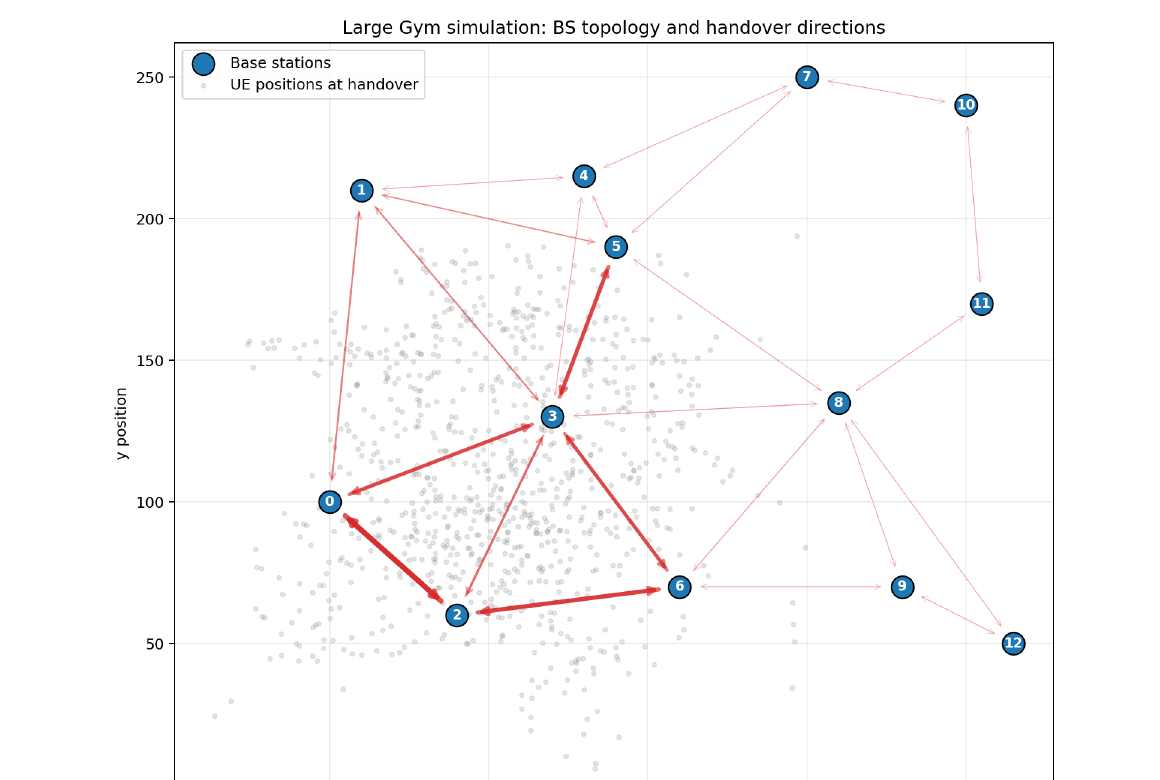
\includegraphics[width=0.9\linewidth]{simulation_engine_plot_original.png}
\caption{Visual outcome of the richer large Gym simulation. Base stations are shown as numbered blue points, sampled UE positions at handover time appear in gray, and red arrows indicate directed handover links observed or added through the richer nearest-neighbor coverage mechanism.}
\label{fig:simulation_engine}
\end{figure}

\subsection{Feature Extraction from Simulation Steps}
For each base station, the simulation records load, average velocity of connected users, number of users in range, average SNR, minimum SNR, and trajectory probabilities toward other base stations. For each directed edge, it records handover count, transition probability, current CIO value, normal handovers, failure counts, and severity values. The edge feature list is now defined directly in \texttt{recursive\_gnn\_cio\_optimization.py} as \texttt{EDGE\_FEATURE\_COLUMNS}.

A major correction was needed in the graph-loading stage. Some SNR values and derived features became non-finite during early experiments, causing NaN losses during training. We therefore added sanitization at several levels. SNR values are clipped and converted to finite values in the simulator. Node features, edge attributes, and target tensors are also passed through finite-value safeguards before being converted to PyTorch tensors. This change was essential for stable training on the larger environment.

\subsection{Failure Detection and Severity Metrics}
The final failure labels are computed directly at handover time. The too-early flag is activated when the new SNR is lower than the old SNR by more than the configured threshold. The too-late flag is activated when the old SNR is below the configured late-handover threshold. The ping-pong flag is activated when the user returns to a previous source-destination pair within a configurable window.

The severity values make the target richer than simple binary classification. The early severity increases with the SNR drop after handover. The late severity increases when the previous serving SNR is below the late threshold. The ping-pong severity is larger when the return handover occurs quickly. The global failure severity is the sum of these components.

The severity quantities are computed with positive-part functions so that only harmful deviations contribute to the score:
\begin{align}
s_E(e)&=\max(0,S_i(e)-S_j(e)-\tau_E),\\
s_L(e)&=\max(0,\tau_L-S_i(e)),\\
s_P(e)&=y_P(e)\left(1-\frac{\min(\Delta t_{return}(e),W)}{W}\right).
\end{align}
The total severity used for continuous targets and CIO adaptation is then
\begin{equation}
s_{fail}(e)=s_E(e)+s_L(e)+s_P(e).
\end{equation}

\subsection{Richer Simulation and Coverage Control}
The first simulations produced sparse CIO matrices. This was initially confusing because the large environment was expected to produce a 19 by 19 matrix with many active values. We later found two separate reasons. First, the code used a hardcoded mapping from environment names to base-station counts, while the actual loaded environments reported fewer base stations. The medium central environment reported 7 base stations and the large central environment reported 13 base stations. The unused rows and columns were therefore artifacts. This was fixed by adding direct detection of \texttt{NUM\_STATIONS} from the Gymnasium environment.

Second, even after correcting the matrix size, realistic mobility does not produce handovers between all possible base-station pairs. A user usually moves between neighboring cells, not between every pair of cells in the network. This remains visible in the final CIO matrices: active rows and local directed pairs receive updates, while unrelated directed pairs can remain zero. This is not considered a failure of the method, but a property of the simulated handover graph.

\section{Complete Training Pipeline}
\label{sec:training_pipeline}

\subsection{Iteration Loop}
The training loop starts from a zero CIO matrix or from a loaded matrix. For each iteration, it runs the simulation, saves graph CSV files, loads graph snapshots, trains a directed GNN, predicts edge risks, updates the CIO matrix, and saves the new matrix and plots. The loop is not a direct gradient descent over CIO values. Instead, the model predicts risk, the risks are compared within each source base-station row, and CIO values are moved according to the relative risk of each outgoing edge.

The current CIO update is row-wise and mean-centered:
\begin{equation}
\Delta CIO_{i,j}=\eta\left(\hat r_{i,j}-\frac{1}{|\mathcal{N}_i|}\sum_{m\in\mathcal{N}_i}\hat r_{i,m}\right).
\end{equation}
After this update, the row is centered again, the diagonal is kept at zero, and values are clipped. This replaced an earlier update rule that could either keep CIO at zero through safety rejection or suppress handovers too strongly.

\subsection{GNN Model Training}
The GNN is trained either as a classifier or as a regressor depending on the target in the legacy pipeline. For classification targets such as \texttt{any\_failure} or \texttt{ping\_pong}, the implementation used weighted binary cross-entropy because accuracy was misleading in the early experiments. When failures are rare or imbalanced, a model can obtain a high accuracy by mostly predicting the majority class. Weighted loss and additional metrics such as precision, recall, F1-score, positive rate, and predicted positive rate provide a more honest evaluation.

The current recursive optimizer trains the GNN as a directed-edge risk regressor. The model output is passed through a sigmoid and optimized with weighted mean squared error:
\begin{equation}
\mathcal{L}=\frac{\sum_{i,j}w_{i,j}(\hat r_{i,j}-r_{i,j})^2}{\sum_{i,j}w_{i,j}},
\end{equation}
where active handover edges receive larger weight than inactive edges. This produces a continuous risk signal that can be converted into CIO adaptation.

\subsection{Rule-Based Component vs. GNN Model}
The pipeline contains two distinct roles that serve different purposes in the closed-loop system. The rule-based component consists of the A3 handover mechanism embedded in the simulator and the deterministic event classification logic that runs after each simulation step. This rule-based component acts as the teacher that generates labels and targets. It provides the actual handover decisions under the current CIO matrix, observes the real handover outcomes with their associated SNR values and timing, and classifies each event as normal, too-early, too-late, or containing ping-pong behavior. From these classified events, the rule-based component computes empirical risk targets at the directed-edge level as $r_{i,j}^{observed} = \frac{f_{i,j}}{h_{i,j}}$, where $f_{i,j}$ is the count of failures on the directed edge from base station $i$ to base station $j$ and $h_{i,j}$ is the total count of handovers on that edge.

The GNN serves as the student model that learns from the rule-based observations. It receives graph snapshots representing the current network state, with node features capturing base-station properties and edge features capturing handover statistics and the current CIO values. The GNN then learns to predict edge-level risk: $\hat{r}_{i,j} = \sigma(f_\theta(G, e_{i,j}))$. This separation of roles is crucial for understanding how the system works. The GNN does not replace the A3 handover rule or the event classification logic. Instead, it learns a statistical relationship between network state and handover risk, and then its predictions modify the CIO matrix used in the next recursive iteration. In this way, the rule-based component defines what happened during the current iteration, and the GNN learns to anticipate what might go wrong in future iterations. The two components form a feedback loop where simulation provides ground truth, the GNN learns from that ground truth, and GNN predictions guide the next simulation run.

\subsection{Online CIO Update}
The older iterative pipeline also supported online CIO updates during a simulation episode. Recent handover events were collected and periodically converted into edge risks. If an edge produced too-early, too-late, ping-pong, or high-severity events, its CIO was decreased to make future handovers along that directed edge less attractive. This mechanism was useful during development because it verified that CIO values could be modified during simulation and that handover labels could be translated into control actions. However, it also made the interpretation of the final matrix more difficult, because CIO values could change both inside an episode and between two GNN training iterations.

For the final framework, the main mechanism is therefore not the online update but the recursive simulator-in-the-loop update. At the end of an iteration, the GNN predicts a directed risk matrix. This risk matrix is converted into a candidate CIO matrix, and the candidate is then tested by re-running the simulator. The safety mechanism does not immediately accept the full update. It first tries the complete candidate, then progressively smaller fractions of the same update, down to very small steps and finally to no update at all. This backtracking procedure was introduced after observing that coarse updates could remove too many handovers and force the optimizer back to an all-zero matrix. In the final presets, a candidate is accepted only if it preserves at least 90\% of the baseline handovers. The result is a more conservative but much more interpretable control loop: the GNN proposes a direction, the simulator tests whether this direction is operationally safe, and only the largest acceptable update is retained.

\section{Data Generation Methodology and Challenges}
\label{sec:data_generation}

\subsection{Simulation Fidelity}
The simulation is useful for prototyping, but it remains a simplified model of a cellular network. The environment uses simplified mobility and channel behavior rather than real traffic traces, urban propagation, device heterogeneity, or temporal load variations. This limitation affected the results. SNR values often became very close to zero after sanitization, and the failure thresholds therefore had to be tuned carefully. The final results should be interpreted as evidence that the pipeline works technically, not as proof of deployment-ready performance.

\subsection{Development History and Corrections}
The first important problem was the dominance of ping-pong failures. This led to the introduction of independent failure flags and continuous severity metrics. The second problem was that high validation accuracy did not necessarily mean good failure detection. This led to weighted binary cross-entropy and additional classification metrics. The third problem was numerical instability. Some runs on the medium and large environments produced NaN losses, so SNR values and graph tensors had to be sanitized and clipped.

The fourth problem was environmental mismatch. We initially believed that \texttt{mobile-medium-central-v0} had 9 base stations and \texttt{mobile-large-central-v0} had 19 base stations. In practice, the installed Gym environments reported 7 and 13 base stations respectively. The matrices therefore contained unused rows and columns. We fixed this by detecting the true base-station count directly from the environment. The fifth problem was CIO sparsity. Even with all base stations present, many directed pairs naturally had no handovers.

A later problem was that recursive GNN CIO updates either stayed exactly zero or collapsed handovers. This was not a plotting issue: the safety gate was rejecting disruptive candidate matrices. The final correction was to use row-wise mean-centered CIO updates, finer safety backtracking, a strict handover-preservation ratio, and a separate display/effective scale so that the stored CIO values are readable while their actual A3 impact remains controlled.

\subsection{Recursive CIO Update Strategy}
The GNN predicts edge-level risk values for each possible directed handover path, but these predictions must then be converted into a new CIO matrix. A naive approach would be to apply a per-edge update: $\Delta CIO_{i,j} = -\eta \cdot \hat{r}_{i,j}$. However, this approach has a critical flaw. If many predicted risks are high, many CIO penalties accumulate on the outgoing edges from a source base station $i$. Users may then find that all outgoing edges from $i$ become unattractive, preventing any handover away from $i$. This causes handover starvation, where users remain connected to degrading cells simply because the CIO penalties are too high everywhere else.

The solution is to use row-wise, mean-centered CIO updates that rank outgoing target risks within each source base station row. The update formula is
\begin{equation}
\Delta CIO_{i,j} = \eta \left( \hat{r}_{i,j} - \frac{1}{|\mathcal{N}_i|} \sum_{m \in \mathcal{N}_i} \hat{r}_{i,m} \right),
\end{equation}
where $\mathcal{N}_i$ is the set of all possible target base stations from source $i$. This formulation creates a competition among outgoing edges: higher-risk targets receive larger CIO penalties, while lower-risk targets receive smaller penalties or even rewards. The row-wise mean-centering ensures that the average CIO from any source base station remains approximately constant, which preserves at least one attractive outgoing direction from that source. After the update, the row is re-centered, the diagonal (self-loops) is reset to zero, and all values are clipped to prevent extreme magnitudes.

Before accepting a candidate CIO matrix generated by this update rule, a safety gate simulates the new handover behavior on a fixed test scenario. If the candidate CIO matrix produces fewer handovers than required, the update is progressively reduced through backtracking factors $(1.0, 0.5, 0.25, 0.1, 0.05, 0.02, 0.01, 0.005, 0.001, 0.0)$ until the updated CIO either meets the handover-preservation threshold or is rejected entirely. In the current presets, an accepted CIO matrix must preserve at least 90\% of the baseline handovers. This safety gate prevents trivial solutions where the GNN-updated CIO would suppress all handovers in the name of avoiding failures. The result is a more conservative but much more interpretable control loop: the GNN proposes a direction through its risk predictions, the simulator tests whether this direction is operationally safe, and only the largest acceptable update is retained.

\subsection{Interpretation of Zeros in the CIO Matrix}
A zero in the final CIO matrix does not necessarily mean a modeling failure. It often means that the corresponding directed pair did not receive handover evidence, or that the source base station did not actively participate in the simulated handover graph. Inactive pairs remain zero. This behavior is preferable to artificially changing all matrix entries, because CIO should mainly be learned for plausible neighboring handover paths.

\section{Experimental Results}
\label{sec:experiments}

\subsection{Experimental Setup}
The final experiments use the recursive optimizer on two environments from the installed \texttt{mobile-env} package. The small experiment uses \texttt{mobile-small-central-v0}, while the large experiment uses \texttt{mobile-large-central-v0}. These two cases were chosen because they test different aspects of the method. The small environment is easier to interpret visually and is useful for checking whether the recursive update produces nonzero CIO values without destroying the handover process. The large environment is more demanding because it contains thirteen detected base stations and therefore a much larger directed CIO matrix.

Both final experiments use fixed scenarios during CIO candidate evaluation. This means that the baseline CIO matrix and each proposed CIO matrix are tested on the same mobility and signal trajectory. This choice is important because otherwise the optimizer could appear better or worse simply because the simulated users followed a different random path. The final small run uses four recursive iterations, short episodes of thirty steps, and two GNN training epochs per iteration. The final large run uses five recursive iterations, longer episodes of eighty steps, and three GNN training epochs per iteration. In both cases the stored CIO values are made readable by using a high CIO learning rate and a wide clipping interval, while the actual impact on the A3 handover condition is controlled by the small effective scale $s_{CIO}=10^{-6}$. The same safety rule is used in both environments: an accepted CIO matrix must preserve at least 90\% of the baseline handovers.

\subsection{Medium Richer Validation}
The medium richer validation from the earlier stage remains useful as a debugging milestone. It verified that the simulation controls, environment-size detection, and graph extraction were functioning before larger runs. The corrected medium matrix had shape 7 by 7. All 7 source base stations and all 7 destination base stations were covered. This result is kept as methodological context, but it is no longer the main final result.

\subsection{Parameter Presets: Small-Balanced vs. Large-Balanced}
To handle the different characteristics of small and large environments, two parameter presets were developed. The script automatically selects the appropriate preset based on environment name when invoked with \texttt{--parameter-preset auto}. The small-balanced preset is used for \texttt{mobile-small-central-v0} and applies relatively conservative SNR gain windows and failure-ratio thresholds: $\texttt{valid\_snr\_gain\_min} = 0.05$, $\texttt{valid\_snr\_gain\_max} = 10.0$, $\texttt{too\_early\_ratio} = 0.70$, $\texttt{too\_late\_ratio} = 4.5$. The large-balanced preset is used for \texttt{mobile-large-central-v0} and applies wider SNR gain windows and different threshold ratios to accommodate the more complex topology and greater diversity of handover scenarios: $\texttt{valid\_snr\_gain\_min} = 0.02$, $\texttt{valid\_snr\_gain\_max} = 25.0$, $\texttt{too\_early\_ratio} = 0.60$, $\texttt{too\_late\_ratio} = 12.0$. Both presets share the same core learning parameters: $\texttt{cio\_lr} = 2000.0$, $\texttt{max\_cio\_step} = 2.0$, and $\texttt{min\_handover\_ratio} = 0.9$. The rationale for different SNR windows is that the large environment exhibits more extreme SNR variations and longer handover distances, so the thresholds must be more permissive to avoid labeling most handovers as failures.

\subsection{Large Richer Diagnostic}
The richer large diagnostic also remains useful for interpreting coverage. It showed that the installed large central environment reports 13 actual base stations rather than the originally assumed 19. It also demonstrated that a CIO matrix should not be expected to be fully dense: many cell pairs do not exchange handovers under realistic local mobility.

The current final large recursive run follows the same lesson. The detected CIO matrix has shape $13 \times 13$, which corresponds to the true number of base stations reported by the environment. With the baseline matrix, the fixed scenario produces 812 handovers. After recursive CIO optimization, the final matrix still produces 773 handovers, corresponding to a handover preservation rate of 95.2\%. This is an important result because it shows that the optimizer did not simply reduce failures by preventing users from changing cells. Although the full matrix contains 60 nonzero entries, only five source base stations actively contribute learned CIO rows in the fixed scenario. For this reason, the most informative visualization is not the full dense topology, but the submatrix restricted to observed handover edges. In that view, values range from -0.180 to 0.367 and reveal the directed structure learned by the recursive optimizer.

\subsection{Training and CIO Results}
The final result folders are \texttt{results\_recursive/final\_small\_cio\_fixed} and \texttt{results\_recursive/final\_large\_cio\_fixed}. They contain the final CIO matrices, predicted risk matrices, handover event logs, failure distribution plots, recursive metrics, and a baseline-versus-GNN comparison file.

For the small environment, the final handover distribution is 85.7\% normal and 14.3\% too-late handovers, with a ping-pong overlay rate of 10.7\%. The final run preserves 28 handovers out of 29 baseline handovers and produces CIO values between -0.101 and 0.101.

For the large environment, the final handover distribution is 74.5\% normal and 25.5\% too-late handovers, with a ping-pong overlay rate of 12.4\%. The final run preserves 773 handovers out of 812 baseline handovers and produces CIO values between -0.180 and 0.367.

\begin{figure}[h]
\centering
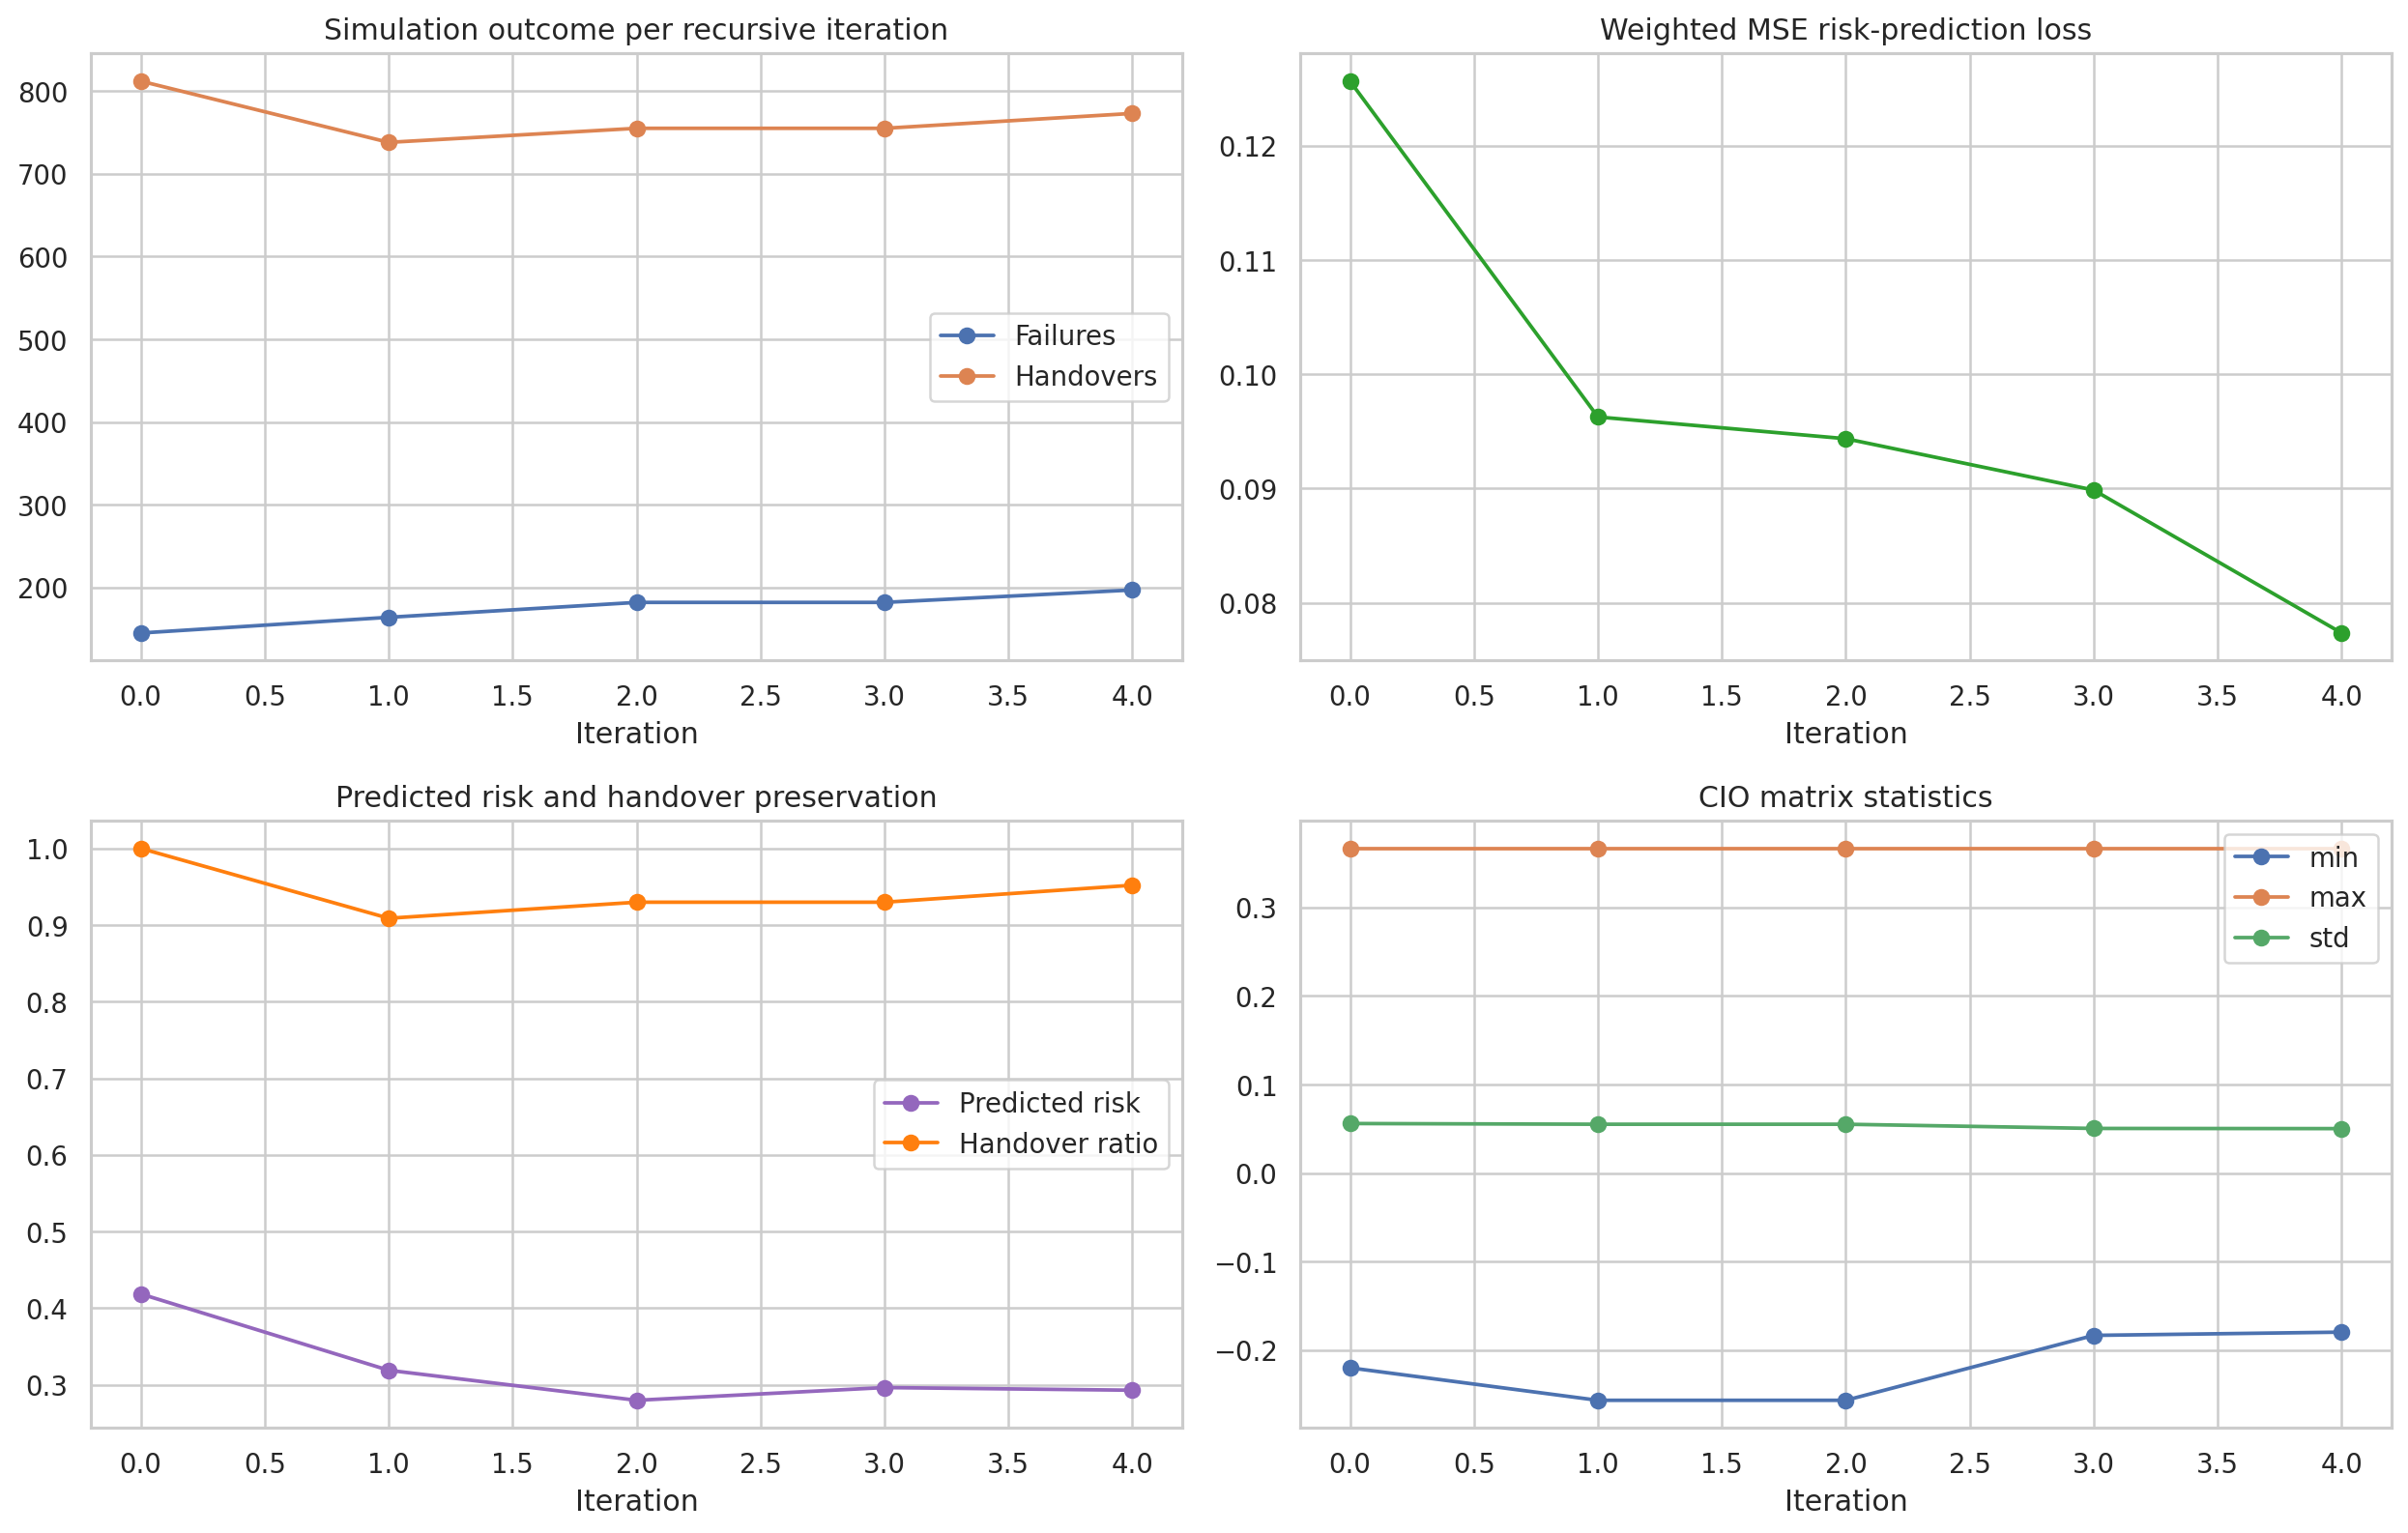
\includegraphics[width=0.95\linewidth]{figures/large_optimization_metrics.png}
\caption{Recursive optimization metrics for the large environment. The plots summarize the evolution of handover preservation, failure count, training loss, predicted risk, and CIO matrix statistics across recursive iterations.}
\label{fig:large_metrics}
\end{figure}

\begin{figure}[h]
\centering
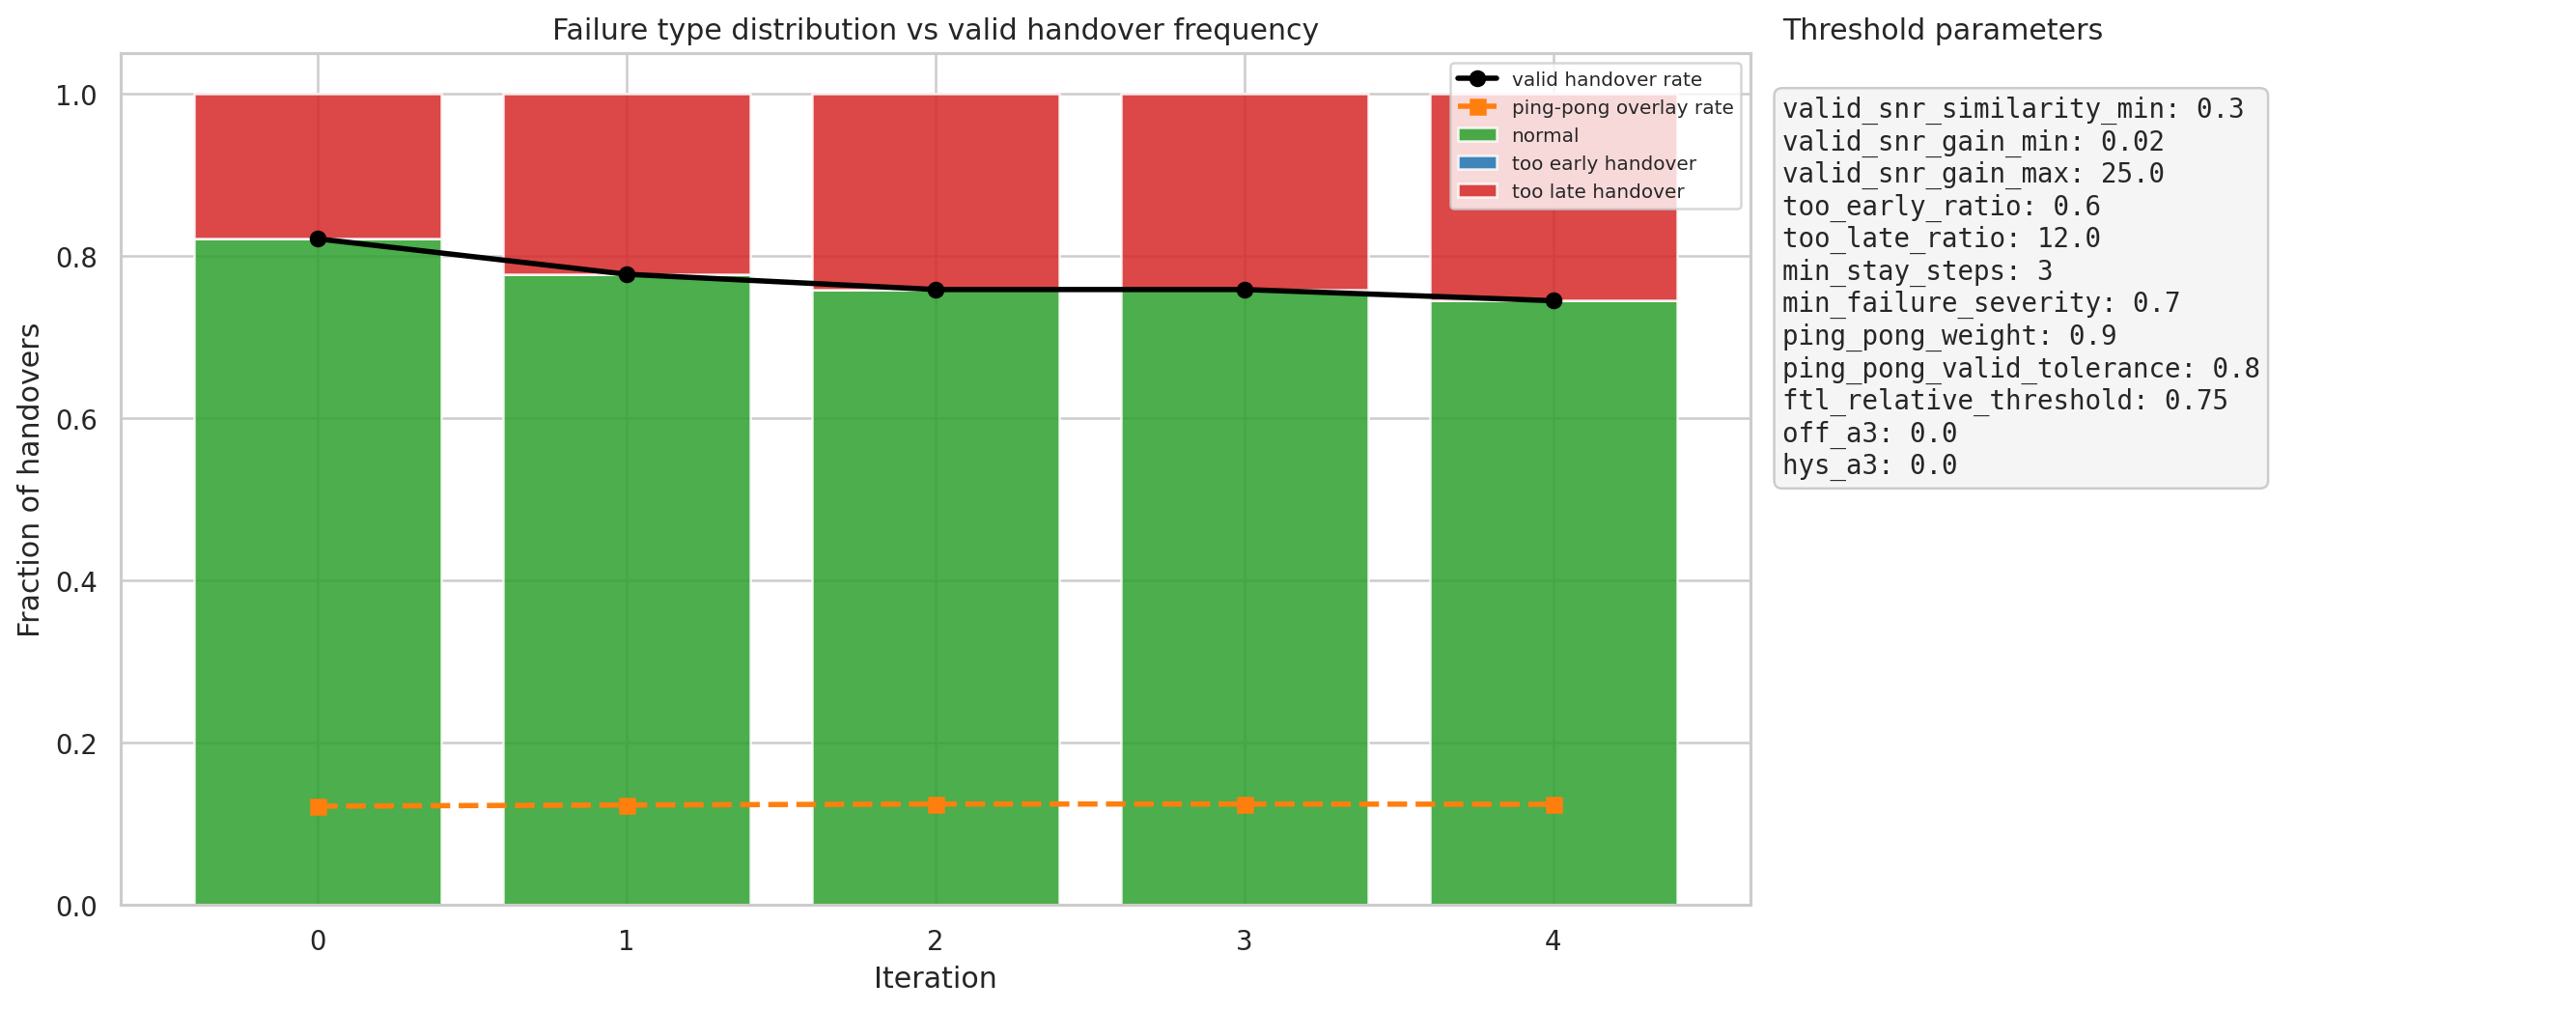
\includegraphics[width=0.95\linewidth]{figures/large_failure_distribution.png}
\caption{Failure-type distribution for the large recursive experiment. The stacked bars show the primary handover classes, while the overlay curves report the valid handover rate and ping-pong rate.}
\label{fig:large_failure_distribution}
\end{figure}

\subsection{Evaluation Protocol and Improvement Indicators}
The recursive loop can be considered to be improving if, over iterations, the failure count decreases or remains controlled, the normal handover rate increases, the total handover count stays above the preservation threshold (90\%), the training loss decreases or stabilizes, the predicted risk matrix exhibits meaningful structure rather than uniform values, the CIO matrix becomes asymmetric in directions that receive handover evidence, and the safety gate indicates starvation correction infrequently. However, improvement cannot be claimed based on lower failure count alone, because a trivial solution could reduce failures by suppressing all handovers. The correct evaluation criterion is that the failure rate is lower or stable while maintaining handover preservation: $\text{(lower failure rate) AND (handover preservation ratio} \geq 90\%)$.

A rigorous evaluation protocol compares three baselines on the same fixed scenario. The first is static A3 with zero CIO, which serves as iteration-0 baseline. The second would be a static rule-based CIO if implemented separately, and the third is the GNN-recursive CIO after the final iteration. For each method, the comparison includes total handover count and the handover preservation ratio, the failure distribution with normal, too-early, and too-late rates, the ping-pong overlay rate, the CIO matrix asymmetry measured as a function of the difference between $|CIO_{i,j}|$ and $|CIO_{j,i}|$, and the mean predicted versus observed edge risk. Additionally, the mean training loss, stability of the predicted risk matrix, and sparsity of the final CIO matrix provide diagnostic signals about the quality of learning and the reasonableness of the proposed CIO values.

\subsection{Diagnostic Runs: Safe vs. Unconstrained Evaluation}
To understand whether the GNN is learning meaningful risk predictions and to diagnose potential issues with the CIO update strategy, two diagnostic runs were performed on \texttt{mobile-large-central-v0} using identical fixed scenarios. In the safe evaluation run, the safety gate was enabled with $\texttt{min\_handover\_ratio} = 0.9$, meaning that CIO updates were accepted only if handovers were preserved above 90\%. The GNN correctly learned the risk target, as evidenced by training loss decreasing from 0.1678 to 0.0330, and mean predicted risk decreasing from 0.4151 to 0.1023. This indicates that the model converged to a reasonable solution. However, despite successful training, the final CIO matrix remained zero because the risk-to-CIO conversion was too disruptive for the handover-preservation constraint. Each candidate CIO update proposed by the recursive update rule caused too many handovers to disappear, so the safety gate repeatedly backtracked the update until it reached exactly zero.

In contrast, an unconstrained diagnostic run was performed with $\texttt{min\_handover\_ratio} = 0.0$, which disables the handover-preservation constraint entirely (this setting is not recommended for production use). In this run, the GNN produced nonzero CIO values scaled on the order of $10^{-4}$ to $10^{-5}$. However, the resulting handovers collapsed from 812 down to 42, representing a 5.17\% preservation rate. The failure distribution worsened substantially: the normal handover rate dropped from 52.34\% to 38.10\%, and the total failure rate increased to 61.90\%. This diagnostic run revealed the root cause of the zero-CIO problem: the risk-to-CIO update rule, in its initial form, was converting high-risk predictions into CIO penalties that were too strong globally.

The solution was to refactor the CIO update mechanism to use the row-wise mean-centered approach described in Section~\ref{sec:data_generation}, which ranks risks within each source-BS row rather than penalizing each edge independently. Additionally, the safety backtracking grid was made finer to allow smaller nonzero CIO updates to be accepted. These changes addressed the fundamental issue: the GNN was learning correctly, but the policy mapping risk to CIO was inherently misaligned with the preservation constraint. After implementing row-wise mean-centering and finer backtracking, subsequent runs on both small and large environments produced meaningful nonzero CIO matrices while maintaining handover preservation.

\begin{figure}[h]
\centering
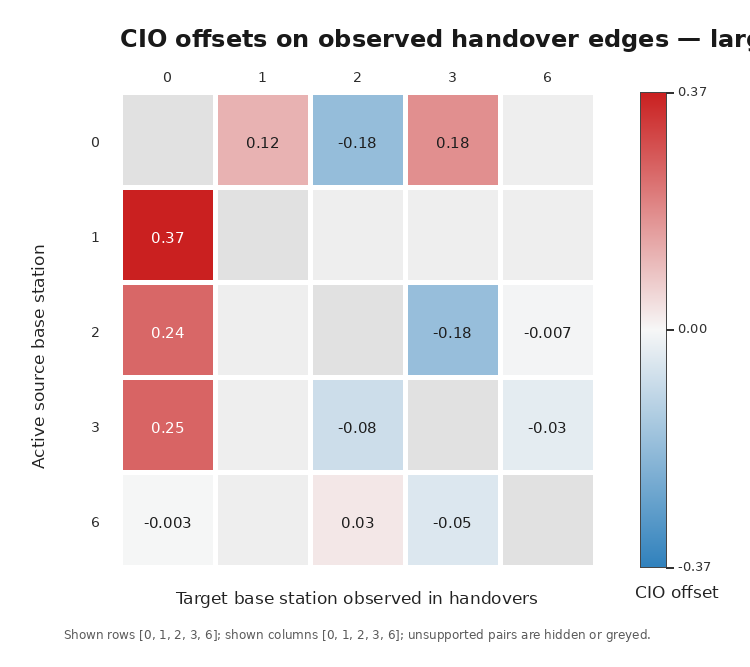
\includegraphics[width=0.82\linewidth]{figures/large_cio_observed_edges.png}
\caption{Final directed CIO offsets on observed handover edges for the large recursive experiment. The figure focuses on base stations that actually participate in learned handover directions, rather than displaying the entire sparse $13 \times 13$ topology. Grey cells correspond to self-links or unsupported directions, while colored cells show the CIO values used by the recursive optimizer.}
\label{fig:large_comprehensive}
\end{figure}

\begin{figure}[h]
\centering
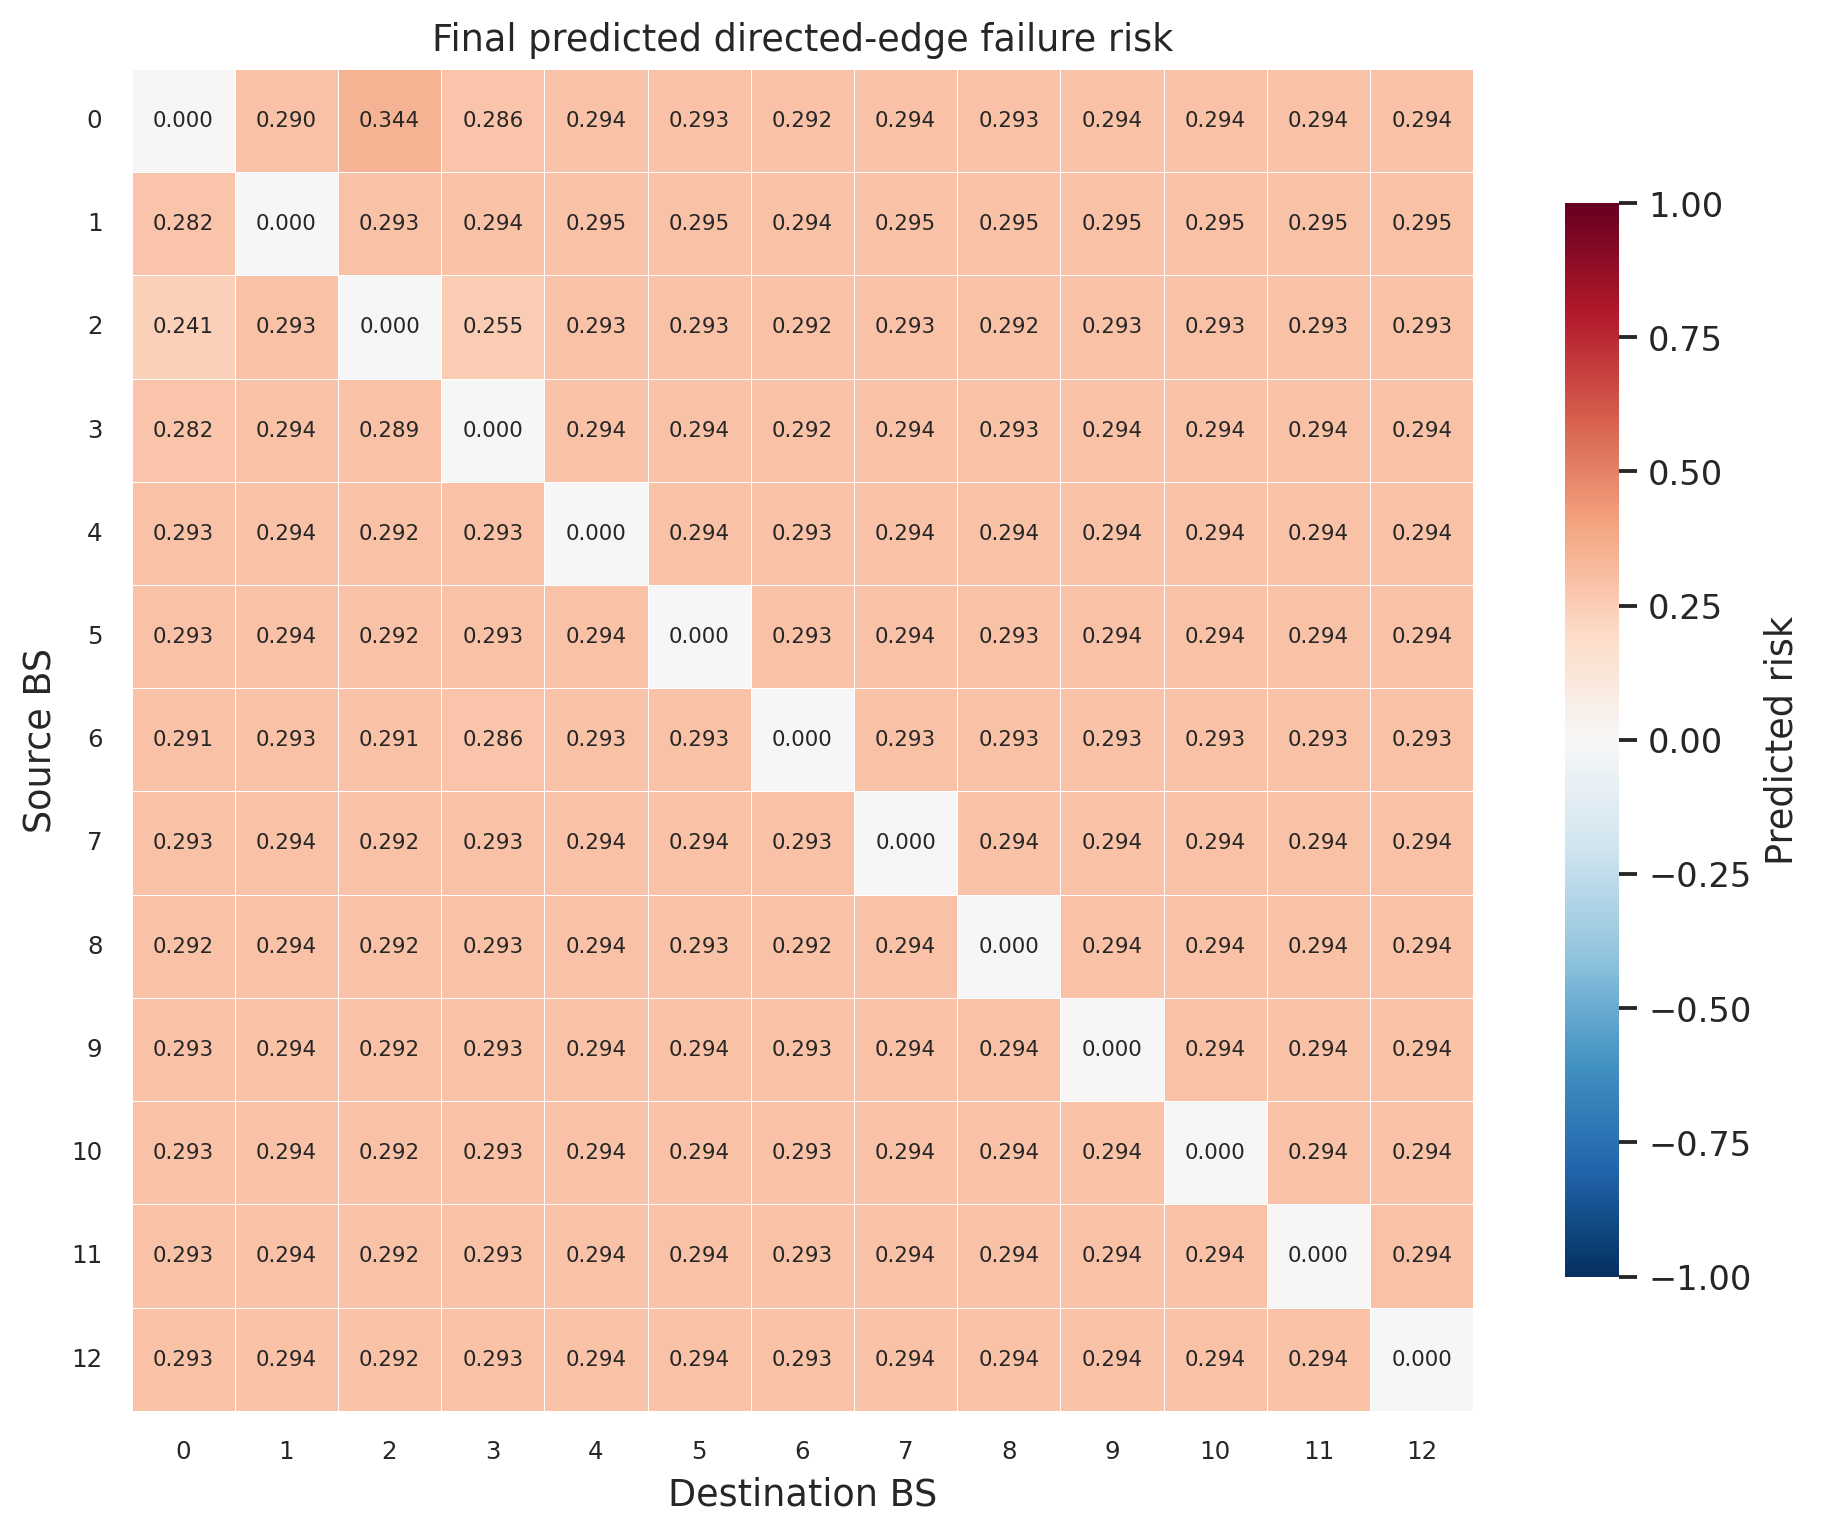
\includegraphics[width=0.82\linewidth]{figures/large_predicted_risk_matrix.png}
\caption{Final predicted directed risk matrix for the large environment. This plot shows the edge-level risk signal produced by the GNN before conversion into CIO offsets.}
\label{fig:large_risk_matrix}
\end{figure}

\begin{figure}[h]
\centering
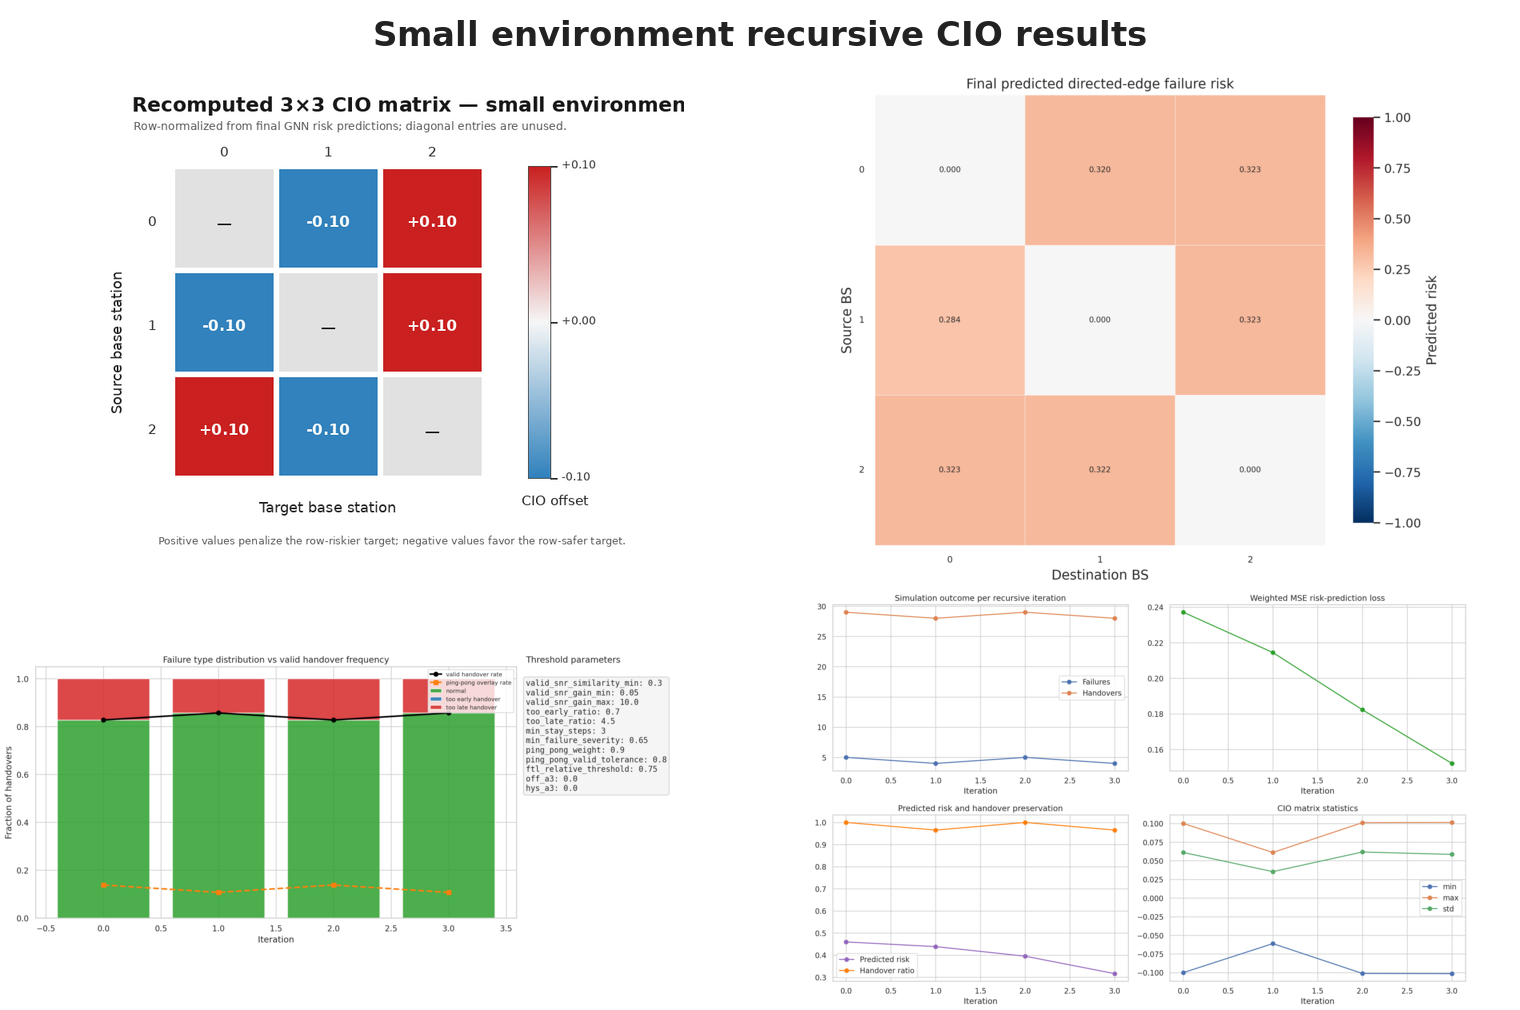
\includegraphics[width=\linewidth]{figures/small_results_panel.png}
\caption{Small-environment recursive CIO result panel. The left plot shows a recomputed row-normalized $3 \times 3$ CIO matrix derived from the final GNN risk predictions, so that each source row compares its two possible targets without leaving inactive entries visually dominant. The remaining plots show the predicted directed risk matrix, the failure-type distribution, and the recursive optimization metrics.}
\label{fig:small_cio_matrix}
\end{figure}

\subsection{Interpretation of the Results}
The final large result is a better representation of the simulated cellular topology than the earlier 19 by 19 matrix. The previous matrix contained many zeros partly because it had unused rows and columns, and partly because not all cell pairs naturally exchange handovers. The corrected version uses 13 actual base stations, but the full matrix is still visually sparse because the fixed scenario does not activate every source base station. In the report, the active-edge CIO view is therefore preferred: it keeps the interpretation focused on handover directions that were actually observed and avoids giving visual importance to unsupported zero entries.

The result also explains why a fully dense CIO matrix is not necessarily desirable. In a realistic spatial network, most handovers should happen between neighboring cells. Forcing every cell to interact with every other cell would make the matrix visually denser, but it would make the simulation less realistic. The final compromise is to allow meaningful nonzero CIO values where the simulator provides evidence and to preserve zeros where the graph has no support.

\section{Limitations and Deployment Considerations}
\label{sec:limitations}
The main limitation is that all results are based on simulation. The simulator is useful for development, but real networks contain additional effects such as building geometry, antenna patterns, interference, scheduler behavior, device differences, and time-varying traffic. The learned CIO values should therefore not be interpreted as directly deployable. They demonstrate that the pipeline can learn and update a directed CIO matrix from simulated data.

Another limitation is the sensitivity of failure labels to thresholds and SNR scaling. Because SNR values had to be sanitized to avoid numerical instability, late failures can become frequent under selected thresholds. This suggests that future work should calibrate thresholds using either real measurements or a more detailed channel model. It may also be useful to train directly on continuous severity targets rather than relying heavily on binary failure definitions.

Finally, the safety gate currently focuses on preserving handover count. This is necessary to avoid handover starvation, but it is not yet a full multi-objective deployment criterion. A real system would need to balance failure rate, ping-pong rate, throughput, load, energy, and operational constraints.

\section{Conclusion}
\label{sec:conclusion}

\subsection{Summary of Contributions}
This project built a complete closed-loop framework for CIO optimization using directed graph neural networks. The final implementation simulates user mobility, records handover events, constructs directed graph snapshots, trains a GNN to predict edge-level risk, and updates a directed CIO matrix. Along the way, the project evolved substantially. We moved from simple failure labels to independent labels and severity metrics, from misleading accuracy to more appropriate loss functions and metrics, from unstable graph tensors to sanitized training data, and from hardcoded matrix sizes to environment-detected base-station counts.

\subsection{Key Findings}
The most important finding is that the CIO matrix should be interpreted through the handover graph. A sparse matrix is not automatically a failure. It may simply reflect that many base-station pairs do not exchange handovers. After correcting the environment size and refining the recursive update, the final large run modifies 60 CIO entries and keeps the remaining unsupported entries at zero. This is more meaningful than a dense matrix filled with artificial values.

The second finding is that debugging the data generation process was as important as training the GNN. The early problems with ping-pong dominance, NaN losses, unused matrix rows, zero CIO values, and handover collapse were not solved by changing the model architecture alone. They required changes in labeling, feature sanitization, CIO update logic, safety acceptance, and simulation design.

\subsection{Future Directions}
The next step would be to make the simulation more realistic without overusing synthetic events. This could include route-based user movement, more diverse user speeds, longer episodes, and calibrated channel models. Another direction would be to evaluate multiple random seeds and tune the large environment closer to an 80\% normal handover rate. The framework could also be extended to optimize additional handover parameters such as hysteresis and time-to-trigger.

\subsection{Final Remarks}
The final system is not only a GNN model but a full experimental pipeline. It shows how a directed graph representation can be used to learn from handover behavior and adapt CIO values. It also shows that careful data engineering is essential. The most useful result of the project is therefore not only the final heatmap, but the understanding of what the entries of the heatmap mean, why many entries should remain zero, and how the simulation can be enriched in a controlled way.

\section*{Acknowledgments}
We are deeply grateful to Alexis Arvanis for his constant guidance during the project. We also highly appreciate the enriching discussions about Graph Neural Networks with his postdoc student, Hiba Hojeij.

\end{document}
